\documentclass[12pt]{article}

% Codificación e idioma
\usepackage[utf8]{inputenc}
\usepackage[spanish]{babel}
\usepackage[T1]{fontenc}
\usepackage{pgfplots}


% Márgenes y estética general
\usepackage[a4paper, margin=2.5cm]{geometry}
\usepackage{lmodern}
\usepackage{setspace}
\usepackage{multirow}
\usepackage{tikz}
\onehalfspacing

% Paquetes matemáticos
\usepackage{amsmath, amssymb, amsthm, mathtools}

%\renewcommand{\thesection}{\Roman{section}}

% Títulos y encabezados
\usepackage{titlesec}
\usepackage[hidelinks]{hyperref}

\title{\textbf{Propuesta de módulos de investigación\\
para el negocio de estaciones de servicio YPF}}
\author{
  Nombre Autor 1\thanks{Afiliación Autor 1} \and
  Nombre Autor 2\thanks{Afiliación Autor 2} \and
  Nombre Autor 3\thanks{Afiliación Autor 3} \and
  Nombre Autor 4\thanks{Afiliación Autor 4}
}
\date{\today}

\begin{document}

\begin{titlepage}
  \centering
  % Título
  {\Large \textbf{Propuesta de módulos de investigación\\
  para el negocio de estaciones de servicio YPF}\par}
  
\vspace{1.5cm}
  
% Autores con afiliación debajo de cada nombre
\begin{center}
\begin{tabular}{cccc}
\large Santiago Cerutti &
\large Guillermo Falcone &
\large Francisco Pizzi &
\large Jorge Puig \\[0.3cm]
\normalsize UNLP--World Bank &
\normalsize CEDLAS--UNLP &
\normalsize UC Davis &
\normalsize UNLP
\end{tabular}
\end{center}

 \vspace{1.5cm} 
  % Fecha en español
  {\large \today\par}


\vspace{2.5cm}

\begin{abstract}
%OLD Esta propuesta presenta un conjunto de módulos independientes de investigación econométrica aplicada para cuantificar el impacto causal de políticas comerciales y operativas de YPF sobre (i) ventas de combustibles, (ii) ventas de tiendas de conveniencia y (iii) participación de mercado a nivel local. Cada módulo está diseñado para producir evidencia accionable para la toma de decisiones del negocio (retail), utilizando diseños de identificación robustos (p.\,ej., diferencias en diferencias con adopción escalonada, estudios de eventos, modelos de panel con efectos fijos y estrategias cuasi-experimentales cuando corresponda). Los resultados permitirán estimar retornos económicos de inversiones (formato FULL, mejoras de infraestructura), evaluar la efectividad neta de promociones y micro-pricing, medir el efecto de innovaciones operativas (autodespacho) y cuantificar el rol de fidelización y alianzas en el margen intensivo (mayor consumo por cliente) y extensivo (captación/retención). Los entregables incluyen estimaciones puntuales con intervalos de confianza, tableros ejecutivos de resultados, y recomendaciones operativas basadas en evidencia para maximizar ventas y rentabilidad.
\end{abstract}
\end{titlepage}

%\begin{itemize}
%  \item \hyperref[block:full]{\textbf{Bloque I: Formato YPF Full y espacios premium}}
%  \item \hyperref[block:promos]{\textbf{Bloque II: Promociones y campañas comerciales}}
%  \item \hyperref[block:pricing]{\textbf{Bloque III: Micro-pricing y estrategias de precios}}
%  \item \hyperref[block:self]{\textbf{Bloque IV: Autodespacho de combustible}}
%  \item \hyperref[block:infra]{\textbf{Bloque V: Infraestructura física e iluminación}}
%  \item \hyperref[block:fidel]{\textbf{Bloque VI: Programas de fidelización}}
%  \item \hyperref[block:segment]{\textbf{Bloque VII: Segmentación de consumidores}}
%  \item \hyperref[block:alliances]{\textbf{Bloque VIII: Alianzas estratégicas}}
%  \item \hyperref[block:competition]{\textbf{Bloque IX: Competencia y participación de mercado}}
%\end{itemize}

\tableofcontents
\newpage


\section{Introducción}

En el mercado minorista de combustibles, el producto principal (naftas y gasoil) es esencialmente homogéneo (sobre todo para la percepción del consumidor promedio), lo que limita la competencia vía precios y desplaza el eje competitivo hacia atributos no--precio: calidad del servicio, experiencia en la estación, programas de fidelización, ubicación y otros servicios complementarios. En Argentina, la evolución reciente del sector muestra que la
participación de mercado dejó de estar determinada exclusivamente por el precio del combustible; factores como la densidad y cobertura de la red, la relación con los franquiciados y la incorporación de servicios de mayor valor agregado —tiendas de conveniencia, oferta gastronómica y \emph{amenities}—
han adquirido un rol central en la dinámica competitiva.

Evidencia econométrica reciente demuestra que las mejoras en la calidad de estos servicios complementarios constituyen un margen competitivo clave en contextos donde la fijación de precios se encuentra restringida o coordinada (Cerutti et al., 2026). En este marco, la estimación rigurosa de efectos causales y de magnitudes económicamente relevantes asociadas a distintas políticas empresariales —tales como inversiones en infraestructura, estrategias comerciales, esquemas de precios, programas de fidelización o innovaciones operativas— resulta fundamental para evaluar su impacto sobre las ventas de combustibles y de tiendas de conveniencia, así como sobre la competencia y la reasignación de demanda entre marcas. Contar con estimaciones precisas de estos efectos permite orientar la toma de decisiones estratégicas en un sector altamente competitivo y de importancia
macroeconómica, evitando conclusiones basadas en correlaciones espurias o análisis puramente
descriptivos.

En los siguientes módulos se detallan distintos análisis econométricos orientados a responder preguntas específicas de relevancia estratégica para el negocio minorista de combustibles y tiendas de conveniencia. Cada módulo está diseñado para cuantificar, de manera rigurosa, el impacto causal de diferentes políticas empresariales sobre las ventas, la composición de la
demanda y la dinámica competitiva entre estaciones. Para cada caso se presenta un enfoque que explicita: (i) el objetivo del análisis, (ii) su justificación económica y relevancia para la toma de decisiones, (iii) el diseño econométrico propuesto, y (iv) los requerimientos de datos necesarios para su implementación.

Los módulos se conciben como proyectos independientes, lo que permite su discusión y ejecución de forma separada, de acuerdo con las prioridades estratégicas de YPF. En todos los casos se privilegiará el uso de metodologías con identificación clara —incluyendo diseños de diferencias en diferencias, modelos de datos de panel con efectos fijos y controles, métodos de \textit{matching}, diseños de regresión discontinua (RDD), estudios de eventos, entre otros, con el objetivo de obtener estimaciones robustas y de interpretación causal válida, evitando conclusiones basadas en correlaciones espurias.





\section{Apertura de Tiendas Full}



\label{block:full}


\subsection{Objetivo}
Cuantificar el impacto de la remodelación de estaciones de servicio al formato \textbf{YPF FULL} —estaciones con tienda de conveniencia modernizada y servicios ampliados— sobre las ventas de combustibles y de la tienda asociada. En particular, se busca estimar en qué
medida la conversión al formato FULL incrementa el volumen de combustible despachado, la facturación total y las ventas de conveniencia, en relación con la trayectoria contrafactual de estaciones comparables que no realizaron dicha inversión. Este grupo de comparación puede incluir tanto estaciones YPF que permanecen en formato tradicional como estaciones de la competencia con características similares (por ejemplo, ubicación, tamaño y tendencia previa de ventas) que no implementan mejoras sustantivas en la calidad de sus servicios durante el período de análisis. 

Adicionalmente, el estudio puede extenderse a la evaluación del beneficio económico neto de la conversión, incorporando información sobre los costos de implementación del formato FULL, tanto de inversión inicial (costos fijos de remodelación) como de operación (costos variables y operativos), lo que permitiría construir métricas de retorno de la inversión y contribuir a la priorización de futuras decisiones de expansión del formato, así como al análisis de la creación de nuevos espacios premium dentro de las estaciones, tales como iniciativas recientemente anunciadas bajo la marca \textbf{YPF Black}.

%\subsection{Justificación y relevancia} La inversión requerida para la remodelación de estaciones de servicio es significativa, por lo que resulta fundamental cuantificar su retorno económico en términos de mayores ventas y márgenes. En particular, las tiendas \emph{Full} se han consolidado como un componente central del negocio, llegando a representar una fracción sustantiva de la rentabilidad de una estación (\textcolor{red}{chequear}). En línea con esta tendencia, YPF ha registrado un fuerte crecimiento en el desempeño de sus tiendas de conveniencia —incluyendo una duplicación de las ganancias en un año y la expansión hasta aproximadamente 1.000 tiendas Full hacia fines de 2024 (\textcolor{red}{chequear})— lo que subraya la relevancia estratégica de este formato.

% Más allá del aumento agregado de ventas, resulta particularmente relevante evaluar si la conversión al formato Full induce una mayor demanda de combustibles \emph{premium}, que presentan márgenes superiores, y si dichos consumidores exhiben patrones de consumo complementarios dentro de la tienda de conveniencia, caracterizados por la compra de productos de mayor calidad y mayor margen. Este canal sugiere un potencial efecto multiplicador de las inversiones en formato Full, al reorientar la demanda hacia segmentos más rentables tanto en combustibles como en productos de la tienda.

% La evidencia disponible para el mercado local respalda la hipótesis de un efecto positivo de las mejoras en servicios complementarios: por ejemplo, se ha documentado que la introducción de estándares gastronómicos en estaciones de servicio incrementó las ventas de combustibles en torno al 10\% en promedio, con aumentos del orden del 20--25\% en las ventas de naftas premium (Cerutti et al., 2026). En este contexto, contar con estimaciones precisas y causalmente identificadas del impacto de la transformación a Full resulta clave para la toma de decisiones. Diferencias en magnitudes aparentemente moderadas —por ejemplo, un aumento del 6\% frente a uno del 9\%— implican variaciones económicamente muy relevantes cuando se las evalúa sobre volúmenes elevados de ventas de combustibles. Por ello, la obtención de coeficientes robustos y bien identificados es esencial para evaluar el retorno de las remodelaciones y optimizar futuras decisiones de inversión, como la priorización de ubicaciones a remodelar o la expansión de formatos premium dentro de la red.

\subsection{Diseño econométrico} Se propone un diseño de \emph{diferencias en diferencias} con tratamiento escalonado (\emph{staggered adoption}) implementado en un marco de \emph{estudio de eventos}, es decir, un único esquema de estimación que combina ambas herramientas siguiendo metodologías de frontera recientes para tratamientos que se adoptan en distintos momentos. En términos prácticos, se compararán las trayectorias de ventas de combustibles y de tienda de las estaciones que se convierten a Full (grupo de tratamiento) antes y después de la remodelación, frente a estaciones que aún no han pasado al formato Full en el mismo período (grupos de control). Este enfoque permite, por un lado, verificar si antes de la intervención los grupos comparados seguían trayectorias similares —una condición necesaria para que la comparación sea confiable— y, por otro, estimar cómo evoluciona el impacto en los períodos posteriores, evitando los sesgos que pueden surgir en métodos de comparación más simples.

Para enriquecer el análisis, se explorarán mecanismos específicos. Por ejemplo, se distinguirá si el aumento en las ventas de combustibles proviene de una mayor afluencia de vehículos (\emph{tráfico}) o de un mayor consumo por cliente (litros por transacción), así como el impacto sobre la mezcla de productos (incrementos relativamente mayores en combustibles premium respecto de los regulares, lo que sería consistente con la atracción de clientes de mayor disposición a pagar). De manera análoga, si se dispone de información pre y post conversión a Full sobre las cantidades vendidas en la tienda de conveniencia —por categoría de producto o incluso a nivel de ítem— se podrá analizar si el formato Full modifica la composición del consumo en la tienda (por ejemplo, hacia productos de mayor calida y margen unitario), complementando así la evidencia sobre el canal de servicios adicionales.

Adicionalmente, se podrá variar sistemáticamente la definición de los grupos de control —considerando distintos conjuntos de estaciones YPF comparables y, cuando los datos lo permitan, estaciones de la competencia similares en ubicación y tendencia previa— con el objetivo de evaluar la robustez de los resultados frente a diferentes contrafactuales plausibles.

\subsection{Datos requeridos} Datos a nivel de estación de servicio con periodicidad mensual (o, preferiblemente, diarios si estuvieran disponibles) que incluyan el volumen de combustibles vendidos —desagregado por tipo de combustible (por ejemplo, nafta súper, nafta premium, gasoil grado 2 y gasoil grado 3)— y los ingresos totales (mensuales o diarios) de las tiendas de conveniencia para cada estación. Para el análisis básico de combustibles, esta información puede obtenerse a partir de los datos administrativos disponibles en la Resolución del Ministerio de Energía, que permiten construir paneles de ventas por estación y mes \textcolor{red}{Alguna oración que diga que es preferible con sus datos porque los del ministerio tienen muchos errores de carga}. Asimismo, se requiere el listado de estaciones con la fecha de remodelación y conversión al formato Full (historial de implementación). \textcolor{red}{esto ya fue provisto por YPF}

Para análisis más detallados y de mayor profundidad, resulta deseable complementar esta información con datos operativos internos de YPF. En particular, contar con variables a nivel de transacción o, alternativamente, con información agregada sobre el número de transacciones y la cantidad total de litros vendidos por período permitiría distinguir entre aumentos en el tráfico de clientes y cambios en el consumo promedio por visita (litros por carga). De manera análoga, para la tienda de conveniencia sería valioso disponer de información sobre cantidades vendidas por categoría de producto, número de tickets y ticket promedio, lo que permitiría analizar cambios en la composición del consumo y en la venta de productos de mayor margen.

Adicionalmente, se podrán incorporar variables de control relativas a las características de la estación (capacidad instalada, número de surtidores, ubicación urbana o sobre rutas) y, cuando sea posible, indicadores del entorno económico o de tráfico vehicular. En caso de extender el análisis a la dimensión competitiva, sería útil contar también con información sobre ventas de combustibles de estaciones de la competencia en la misma zona, ya sea a partir de fuentes públicas, datos administrativos o estimaciones de mercado disponibles.









\section{Programa de Fidelización \emph{Serviclub}}
%
%\section*{Bloque F: Evaluación del programa de fidelización (márgenes intensivo vs. extensivo)}


% Serviclub es el programa de fidelización. LA APP no es Serviclub, sino una herramienta para usar Serviclub, en donde acumulás y canjeas puntos por descuentos, productos o beneficios. Existen Cliente Serviclub que NO usan la app, a YPF le conviene que usen la App porque le permite trackear mejor el consumo y habilita marketing personalizado.

\subsection{Motivación}
Los programas de fidelización no solo buscan retener clientes: también generan datos valiosos sobre comportamiento de consumo y respuesta a incentivos. Sin embargo, el hecho de que los socios consuman más que los no socios no implica que el programa cause ese mayor consumo. Puede simplemente reflejar que quienes más cargan nafta son también quienes más se afilian. El objetivo de esta propuesta es ir más allá de esa comparación descriptiva y estimar el efecto causal del programa sobre ventas, mix de productos y márgenes.
Para eso planteamos una batería de tres ejercicios complementarios, cada uno diseñado para aislar un aspecto distinto del impacto de Serviclub. Los tres pueden implementarse en conjunto y sus resultados se refuerzan mutuamente.

\subsection{Objetivos}
Las preguntas centrales que guían el análisis son:


\begin{itemize}
    \item ¿El programa aumenta la frecuencia de carga y consumo de sus socios, o solo los atrae porque ya cargaban más?
    \item ¿Qué tipo de beneficios generan mayor consumo adicional?
    \item ¿La variedad de productos que consumen difiere entre socios y no socios?
    \item ¿Los socios responden más a mejoras en la experiencia de la estación que los no socios?
    \item ¿La fidelización se explica por los beneficios del programa, o por la experiencia integral de compra?
    %\item ¿Qué campañas logran \emph{fidelizar} a los clientes?
\end{itemize}

\subsection{Diseño general}
El desafío metodológico principal es que la base de datos de \emph{Serviclub} registra el consumo una vez que el cliente ya es socio, pero no antes de su afiliación. Esto impide, en principio, comparar directamente el comportamiento de cada cliente antes y después de unirse al programa\footnote{En caso de que las bases de transacciones cuenten con datos de tarjetas de crédito/débito que permitan trackear clientes no-socios existirían más alternativas.}.
Sin embargo, la combinación de datos transaccionales, uso de beneficios e implementación de campañas permite diseñar tres ejercicios cuasi-experimentales que sortean esta limitación de maneras distintas y complementarias. 

\subsubsection*{Ejercicio 1: El efecto de canjear premios sobre el consumo posterior}
\textbf{Pregunta:} ¿Redimir una recompensa (canje de puntos, descuento, beneficio) aumenta la frecuencia de carga u otros consumos en los meses siguientes?

\textbf{Lógica del ejercicio:} Dentro del universo de socios, no todos canjean premios con la misma frecuencia ni en los mismos momentos. Esto genera variación natural que puede aprovecharse: si dos socios con patrones de consumo similares difieren en si canjearon o no un beneficio en determinado mes, podemos comparar su comportamiento posterior.

La estrategia consiste en usar cada evento de canje como un ``experimento natural'' y analizar si el consumo del cliente aumenta en los meses siguientes respecto a su propio historial previo y respecto a socios similares que no canjearon en ese período. Este tipo de análisis, conocido como estudio de eventos, permite aislar el efecto del canje del resto de los factores que afectan el consumo.

Existe evidencia en la literatura de marketing que indica que redimir premios refuerza el hábito de compra: el cliente que canjea recibe una señal concreta del valor del programa, lo que incrementa su compromiso con la marca. Este ejercicio permite testear si eso ocurre en \emph{Serviclub}.

\textbf{Datos necesarios:} Historial de transacciones por cliente con fechas, montos y tipo de producto; registro de canjes con fecha y tipo de beneficio.

\subsubsection*{Ejercicio 2: Campañas de afiliación como fuente de variación}
\textbf{Pregunta:} ¿Los clientes que se afilian al programa por una campaña específica muestran un comportamiento distinto —y más sostenido— que quienes se afilian de forma espontánea?

\textbf{Lógica del ejercicio:} YPF implementa campañas de afiliación en distintos momentos y regiones (por ejemplo, promociones vinculadas a eventos, como las del Mundial). Estos lanzamientos generan "olas" de nuevos socios que se afilian en un período acotado y por un motivo identificable, lo que los hace comparables entre sí y distinguibles de quienes se afilian por iniciativa propia en otros momentos.

La estrategia consiste en comparar la evolución del consumo de dos grupos: los clientes que se afiliaron durante una campaña específica y los que se afiliaron de forma más gradual y espontánea en períodos sin campaña activa, controlando por características observables como estación habitual, tipo de vehículo y nivel de consumo previo estimado.

Si los clientes captados por campaña muestran mayor retención y consumo sostenido, eso indica que la campaña no solo amplía la base de socios sino que atrae perfiles más comprometidos. Si, en cambio, su comportamiento decae rápidamente tras el fin de la campaña, sugiere que el vínculo fue oportunista y no generó fidelización real.

Este ejercicio responde directamente a una pregunta de negocio concreta: ¿vale la pena invertir en campañas de afiliación masiva, o es mejor apostar a la afiliación orgánica?

\textbf{Datos necesarios:} Registro de afiliaciones con fecha y canal (campaña específica vs. espontáneo); historial de consumo post-afiliación; datos de estación y vehículo cuando estén disponibles.


\subsubsection*{Ejercicio 3: Complementariedad entre \emph{Serviclub} y la experiencia en la estación}
\textbf{Pregunta:} ¿Los socios de \emph{Serviclub} responden más a las mejoras en la estación que los no socios? ¿O dicho de otro modo: ¿el programa y la experiencia física se potencian mutuamente?

\textbf{Lógica del ejercicio:} Las remodelaciones de estaciones al formato YPF Full 
representan un cambio significativo en la experiencia de compra ---infraestructura, 
servicios, atención--- sin que el funcionamiento de \emph{Serviclub} se modifique. 
Sin embargo, las estaciones que se remodelan probablemente no son elegidas al azar: 
YPF puede priorizar estaciones con mayor potencial de crecimiento, mejor ubicación o 
determinado perfil de clientes. Esto implica un problema de selección: socios y no 
socios en esas estaciones podrían ser distintos \emph{antes} de la remodelación, lo 
que contaminaría cualquier comparación simple entre estaciones Full y no Full \footnote{Este tema se abordará en profundidad en el módulo correspondiente a la implementación de FULL}.

La estrategia para sortear este problema es agregar la dimensión temporal, comparando 
el comportamiento de cada grupo antes y después de la remodelación dentro de una misma 
estación. Esta metodología ---conocida como \emph{Triple Diferencia}--- controla por 
todas las características fijas de cada estación y de cada cliente, y permite 
identificar el cambio en la brecha entre socios y no socios que ocurre justo cuando 
la estación se remodela, no el nivel absoluto de esa brecha.

En términos concretos, el modelo compara cuatro grupos simultáneamente (ver Cuadro \ref{tab:triple_diff}): socios y no socios, en estaciones Full y no Full, antes y después de la remodelación. El coeficiente clave mide si el efecto de la remodelación sobre el consumo es distinto para socios que para no socios: si la remodelación beneficia por igual a ambos grupos, el efecto se explica por la mejora general de la estación; pero si el aumento es significativamente mayor entre los socios, eso indica que el programa y la experiencia física se potencian mutuamente.

Si se encuentra esa complementariedad, las implicancias para la empresa son dobles.Por un lado, la inversión en remodelaciones Full genera un retorno adicional entre los clientes ya fidelizados por \emph{Serviclub}, lo que fortalece el caso para priorizar esas inversiones en estaciones con alta penetración del programa. Por otro lado, el programa estaría siendo subutilizado en estaciones no Full: los mismos incentivos rinden menos donde la experiencia de compra es de menor calidad. En conjunto, esto sugiere que la expansión de \emph{Serviclub} y la mejora de infraestructura son decisiones que conviene coordinar, y no evaluar de forma independiente.

\textbf{Datos necesarios:} Fechas de remodelación por estación; historial de transacciones distinguiendo socios y no socios; datos suficientes antes y después de cada remodelación para al menos un subconjunto de estaciones.



\begin{table}[h]

\centering
\caption{Estructura de la Triple Diferencia}
\label{tab:triple_diff}
\setlength{\extrarowheight}{4pt}
\begin{tabular}{lcc}
\hline\hline
 & \textbf{Antes de remodelación} & \textbf{Después de remodelación} \\
\hline
\textit{Estación Full} & & \\
\quad Socio Serviclub   & $A$ & $B$ \\
\quad No socio          & $C$ & $D$ \\[4pt]
\textit{Estación no Full} & & \\
\quad Socio Serviclub   & $E$ & $F$ \\
\quad No socio          & $G$ & $H$ \\
\hline\hline
\multicolumn{3}{p{10cm}}{\footnotesize El efecto buscado es: 
$[(B-A)-(D-C)] - [(F-E)-(H-G)]$. 
Si este valor es positivo y significativo, existe complementariedad entre 
el programa \emph{Serviclub} y la experiencia en estaciones Full.}\\
\end{tabular}
\end{table}

\begin{table}[h]
\centering
\small
\setlength{\extrarowheight}{5pt}
\setlength{\tabcolsep}{10pt}
\begin{tabular}{lcccc}
\hline\hline
 & \multicolumn{2}{c}{\cellcolor{corporateblue!12}\textbf{Antes}}
 & \multicolumn{2}{c}{\cellcolor{corporateblue!38}\textbf{Después}} \\
 & \cellcolor{corporateblue!12}\small\textbf{Socio}
 & \cellcolor{corporategray!20}\small\textbf{No socio}
 & \cellcolor{corporateblue!12}\small\textbf{Socio}
 & \cellcolor{corporategray!20}\small\textbf{No socio} \\
\hline
\textit{Estación Full}
 & \cellcolor{corporateblue!22}$A$
 & \cellcolor{corporategray!12}$C$
 & \cellcolor{corporateblue!52}$B$
 & \cellcolor{corporategray!38}$D$ \\
\textit{Estación no Full}
 & \cellcolor{corporateblue!22}$E$
 & \cellcolor{corporategray!12}$G$
 & \cellcolor{corporateblue!52}$F$
 & \cellcolor{corporategray!38}$H$ \\
\hline\hline
\end{tabular}

\vspace{0.6em}
\[
\text{Efecto buscado} =
\underbrace{(B - A) - (D - C)}_{\text{DiD en estaciones Full}}
\;-\;
\underbrace{(F - E) - (H - G)}_{\text{DiD en estaciones no Full}}
\]
{\footnotesize\color{corporategray}\itshape
Tonos más oscuros = período post-remodelación.\quad
Azul: socios \emph{Serviclub}.\quad Gris: no socios.}
\end{table}

\begin{figure}
    \centering
    \caption{Diagrama ilustrativo de la Triple Diferencia}
    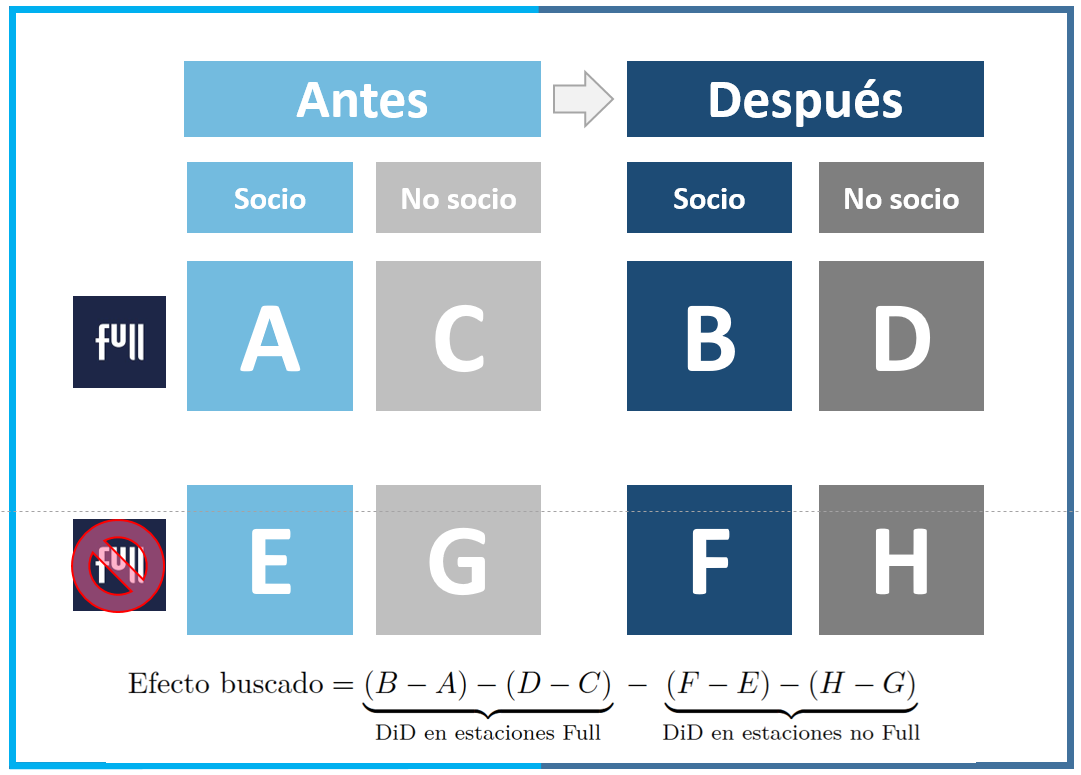
\includegraphics[width=0.6\textwidth]{../../imagenes/esquema_ddd.png}
\end{figure}



\textbf{Modelo base (triple diferencia):}
\[
y_{ist}=\beta_1 Socio_i + \beta_2 Full_{st} + \beta_3(Socio_i\times Full_{st}) + \alpha_i + \gamma_t + \delta_s + \varepsilon_{ist}
\]

donde $y_{ist}$ es el consumo de combustible del cliente $i$ en la estación $s$ y periodo $t$, $Socio_i$ es una variable indicadora de si el cliente es socio de \emph{Serviclub}, $Full_{st}$ indica si la estación $s$ fue remodelada al formato Full en el periodo $t$, $\alpha_i$ son efectos fijos de cliente, $\gamma_t$ efectos fijos de tiempo y $\delta_s$ efectos fijos de estación. Por lo que $\beta_3>0$ sugeriría que \emph{Serviclub} rinde mas donde mejora la experiencia integral.

\subsubsection*{Ejercicios adicionales}
\textcolor{red}{¿Qué campañas o beneficios fidelizan más? Event Study de campañas específicas}


\subsection{Datos requeridos}
Principales bases de datos y variables necesarias para este módulo:
\begin{itemize}
    \item Transacciones de estaciones de servicio: fecha, estación, litros, ticket, tipo de combustible, compras en tienda, método de pago, uso de la App, etc.
    \item Transacciones de clientes \emph{Serviclub}: IDEM anterior pero con identificación de \textbf{Cliente}, para poder construir panel individual.
    \item Información del cliente \emph{Serviclub}: \textbf{Cliente}, fecha de alta, edad, genero, localidad, etc.
    \item Canjes de clientes \emph{Serviclub}: \textbf{Cliente}, fecha, tipo de canje, puntos utilizados, beneficios obtenidos, exposición a campañas, etc.
\end{itemize}

El universo de análisis se definirá más adelante al conocer con más precisión la implementación del programa y campañas. Idealmente abarcaría varios meses o años, para poder observar la evolución del comportamiento de consumo antes y después de la afiliación al programa, así como la respuesta a diferentes campañas e incentivos. Además, será necesario contar con información detallada sobre promociones específicas y campañas ofrecidas dentro del programa, incluyendo fechas de implementación y alcance geográfico de las mismas.


\textbf{Minimo viable:}
\begin{itemize}
    \item panel transaccional de socios (fecha, estacion, litros, ticket, tipo de combustible, compras en tienda);
    \item fechas de alta, uso de App, canjes y exposicion a campanas;
    \item panel mensual por estacion (ventas totales, share \emph{Serviclub}, mix de productos, precios);
    \item calendario de campanas e implementaciones por zona/estacion;
    \item identificacion de remodelaciones Full para el ejercicio de complementariedad.
\end{itemize}




\section{Infraestructura de Comunicación: Cartelería Digital}



\subsection{Objetivo}
    YPF ha implementado \emph{cartelería digital en estaciones}, lo que permite efectuar comunicación comercial dinámica. El objetivo de este bloque se centra en evaluar si esta infraestructura impacta en ventas y qué tipo de mensajes son más efectivos. EN lineas generales, se estimara  cómo ciertas características físicas y de infraestructura de las estaciones de servicio, inciden en las ventas de combustibles y de productos de tienda. Se trata de aislar el efecto de mejorar un atributo físico específico sobre el comportamiento de los consumidores. 
    \begin{itemize}
        \item ¿La cartelería digital aumenta las ventas de la estación?
        \item ¿Qué tipo de promociones funcionan mejor?
        \item ¿Importa el momento del día en que se muestra la promoción?
        \item ¿Influye la ubicación del cartel dentro de la estación?
        \item ¿Genera más cross-selling hacia productos de tienda?
        \item ¿Qué retorno económico tiene la inversión en cartelería digital?
        \item ¿Aumenta el flujo de clientes o el volumen por ticket gracias a un entorno más atractivo y seguro?  
        \item ¿Ciertas mejoras físicas impactan más en las ventas nocturnas o en la captación de cierto perfil de cliente?
    \end{itemize}
    
Este modulo se basa en una secuencia de dos preguntas que se encuentran relacionadas. La carteleria digital esta pensada para mejorar la experiencia del usuario y para aumentar la identificacion entre la marca y el consumidor. Adicionalmente, conidcional en que lo anterior se cumpla, existe una pregunta sobre si estas caracteristicas se traducen en un aumento de ventas. La dificultad en  abordar estas preguntas reside en que se deben separar los efectos por un lado, el impacto en el usuario, y por otro lado el impacto en las ventas. Es decir, es posible que un usuario logre una identificacion mayor con la marca, pero que esto no se traduza en un aumento de combustible u otros serivicios vendidos. 
Una estratgia en donde por ejemplo se encueste a usuarrios antes y despues de la implementacion de la carteleria digital, puede ayudar a medir el impacto en la experiencia del usuario. Sin embargo, uno no podria medir el impacto que esa mejora ha tenido en las ventas. Por otro lado, una estrategia de medicion que intente explicar el aumento de ventas a partir de un aumento en la implementacion,  no necesariamente puede medir el canal por el cual se ha dado ese aumento. Sin conocer el canal, no se puede determinar si el aumento en ventas es por un aumento en la experiencia del usuario, y ahora el consumdidor se fideliza m'as con YPF, o porque la es simplemente un aumento geniuno de la demanda en donde la carteleria digital ha sido implementada, porque  desde antes de la implementacion, esa zona ha tenido un aumento de demanda. Una correcta estrategia de estimacion deberia contemplar las dos cuestiones en simultaneo. 

\subsection{Diseño econométrico}
    Para una estimacion correcta y un analisis integral sobre la implementacion de carteleria digital, se necesita una discusion conceptual con el equipo que se encuentre implementando los conceptos. 
    Los objetivos de la comunicacion comercial dinamica, en general se basan en: 
    \begin{enumerate}
        \item Identificacion del consumidor con la marca.
        \item Experiencia del usuario. 
    \end{enumerate}
    Dentro de los dos puntos anteriores, existen objetivos puntuales. Es decir, en epoca del mundial, una publicidad especifica sobre la seleccion argentina. Una estrategia usual es analizar encuestas a consumidores sobre la relacion con la marca, ejemplo encuestas de calidad de servicio en la estacion de servicvio misma o a traves de \emph{APP YPF}. Dado el nivel desagregado de informacion de la APP, se pueden estimar metricas sobre el impacto de una publicidad especifica en el uso de la Aplicacion. Una primera etapa constaria de individualizar si al cambiar la publicidad, en promedio, la aplicacion se abre mas, o se usa mas tiempo. El hecho de contar con datos a nivel usuario que se pueden linkear con la estacion de servicio donde los clientes cargan combustible genera que se pueda medir que tanto los consumidores interactuan con la aplicacion. 
    La estrategia no se limita a estimar simplemente el impacto de las distintas publicidades en la interaccion del usuario con la aplicacion sino que utiliza ese insumo en una segunda etapa para determinar como la mayor o menor exposicion a la interaccion con la aplicacion genera efectos en la demanda ya sea de combustibles y productos dentro de la tienda. 
    La estrimacion vendria a ser un modelo por variables instrumentales donde la variable instrumental seria la exposicion a la publicidad, que se mide a traves de la interaccion con la aplicacion. La variable endogena seria el aumento en ventas, y el resultado de interes es el impacto de la interaccion con la aplicacion sobre las ventas.
    Los resultados sirven en dos dimensiones. En una primera etapa, se puede rankear el tipo de publicidad a la que los consumidores son mas reactivos, midiendo con una metrica precisa, dada por la interaccion con la aplicacion. POr otro lado, este aumento de interaccion con la aplicacion, puede considerarse exogeno, dado que la publicidad se muestra de manera aleatoria a los consumidores, y entonces estimar de manera causal como la interaccion con la aplicacion se refleja en ventas, ya sea en el momento, o en futuros momentos. 


  \subsection{Datos requeridos}
    
    Para una completa estimacion, se necesitan datos a nivel usuario y anivel estacion de servicio, con frecuencia hora/día. Se necesita informacion sobre los tipos de publicidades mostradas en la carteleria digital.  Por otro lado, se necesitan datos sobre las ventas de combustibles y productos de tienda, con una frecuencia diaria o incluso horaria, para poder medir el impacto de la publicidad en las ventas. Adicionalmente, se necesitan datos sobre la interaccion de los usuarios con la aplicacion, para medir el impacto de la publicidad en la interaccion con la aplicacion. 
    La base de datos ideal tendria una estructura a nivel de estacion de servicio/hora con la cantidad de usuarios que compraron combustible, la cantidad de usuarios que interactuaron con la aplicacion, el tipo de publicidad mostrada en la carteleria digital, y las ventas de combustibles y productos de tienda. 





\section{YPF BOXES (lubricentros)}



\section*{Conclusión}

%OLD La presente propuesta detalla un conjunto de módulos de investigación econométrica aplicada, orientados a proveer información estratégica accionable para YPF en su negocio de estaciones de servicio. Cada bloque aborda una problemática clave –desde la efectividad de inversiones en formato Full o iluminación, hasta el impacto de estrategias comerciales innovadoras como micro-pricing, programas de fidelización y alianzas– con metodologías de punta que garantizan identificaciones causales claras. Al estar estructurados como módulos independientes, estos estudios pueden encararse de manera escalonada según las prioridades del Directorio, manteniendo en todos los casos un estándar técnico-profesional alto y un enfoque práctico en la toma de decisiones. Aplicando estas técnicas modernas de análisis sobre los abundantes datos operativos de YPF, la compañía podrá cuantificar el efecto real de sus iniciativas en un mercado competitivo, separando el \emph{ruido} de la \emph{señal} en la información. De este modo, YPF obtendrá insumos robustos para optimizar sus estrategias de aumento de ventas, mejora de experiencia al cliente y consolidación de su liderazgo de mercado, basados en evidencia empírica concreta adaptada a su realidad de negocio.

\end{document}